\documentclass[a4paper,12pt]{article}


% add more packages if necessary
\usepackage{xspace}
\usepackage{graphicx}
%\usepackage{xcolor}
%\usepackage{hyperref}


% TODO: Add your group name
\newcommand{\groupname}{twitchplayseth\xspace}


\title{
Project Report \\ 
Group \groupname \\
\vspace{5mm}
\large Java and C\# in depth, Spring 2014
}
\author{
% TODO: Add your names here
Leonhard Helminger \\
Marc G\"ahwiler \\
Philipp Gamper
}
\date{\today}



\begin{document}
\maketitle

\section{Introduction}

This document describes the design and implementation of the \emph{Personal Virtual File System} of group \emph{\groupname}. The project is part of the course \emph{Java and C\# in depth} at ETH Zurich. The following sections describe each project phase, listing the requirements that were implemented and the design decisions taken. The last section describes a use case of using the
\emph{Personal Virtual File System}.

% PART I: VFS CORE
% --------------------------------------

\section{VFS Core}

The \emph{VFS Core} provides a basic interface that allows to create and remove a \emph{VFS container file} and perform certain operations on an existing \emph{VFS container file} that are required to fulfill all requirements mentioned in the next section.

The main API classes are 
\begin{description}

\item[VDisk] \hfill\\ Provides an interface to create a new \emph{VFS container file}, delete an existing \emph{VFS container file} or perform certain operations on an existing \emph{VFS container file}.

\item[VDirectory] \hfill\\ Represents a directory in the \emph{VFS}. Provides an interface to get the entries of the directory, add and remove entries and copy or delete the whole directory including it's entries.

\item[VFile] \hfill\\ Represents a file in the \emph{VFS}. Provides an interface to write and read from the file and to copy or delete the file.

\item[VStats] \hfill\\ Provides information about the \emph{VFS}. This includes the size of the \emph{VFS}, used and free space and blocks and the number of directories and files.
\end{description}

\subsection{Requirements}
In this section all requirements, that were implemented in the first part, are listed. For each requirement there is a short description of the requirement and how it is implemented in the project.

\subparagraph{The virtual disk must be stored in a single file in the working directory in the host file system} \hfill\\
The idea behind the virtual disk is to store a virtual file system in a single file in an existing file system (which is called the host file system from now on). This requirement is implemented in \texttt{VDisk}.

\subparagraph{\emph{VFS} must support the creation of a new disk with the specified maximum size at the specified location in the host file system} \hfill\\
A new \emph{VFS} can be created using the \texttt{VDisk} class. To create a new \emph{VFS} it is necessary to format the \emph{VFS file} using the \texttt{format} method of \texttt{VDisk} before it is used for the first time.


\subparagraph{\emph{VFS} must support several virtual disks in the host file system} \hfill\\
Once a \emph{VFS} file has been created and formatted, it can be opened by using the constructor of \texttt{VDisk}. The implementation allows to create and open an unlimited amount of \emph{VFS files} which each contain their own \emph{VFS}. There is no limitation of how many \emph{VFS files} are opened in parallel at runtime (excluding system limitation like amount of available RAM or physical diskspace).

\subparagraph{\emph{VFS} must support disposing of the virtual disk} \hfill\\
A previously created \emph{VFS file} can be deleted with the \texttt{discard} method of \texttt{VDisk}. It simply removes the \emph{VFS file} from the host's filesystem.

\subparagraph{\emph{VFS} must support creating/deleting/renaming directories and files} \hfill\\
All necessary interfaces that handle file/directory creation, deletion and renaming are implemented as methods of \texttt{VDisk}, namely \texttt{touch}/\texttt{mkdir}, \texttt{delete} and \texttt{rename}.

\subparagraph{\emph{VFS} must support navigation: listing of files and folders, and going to a location expressed by a concrete path} \hfill\\
To keep the \texttt{VDisk} class stateless in regard to the current file or directory, the \texttt{VDisk} class provides a \texttt{resolve} method that expects a path in the \emph{VFS} and returns a \texttt{VDirectory} instance if the path is valid. To list the files and sub-directory, that a directory contains, the \texttt{list} method of \texttt{VDisk} can be used in combination in a previously resolved \texttt{VDirectory}.

\subparagraph{\emph{VFS} must support moving/copying directories and files, including hierarchy} \hfill\\
To move or copy a \texttt{VDirectory} or \texttt{VFile} in the \emph{VFS} there exist the \texttt{move} and \texttt{copy} methods in the \texttt{VDisk} class. Both methods support both copying/moving a \texttt{VDirectory}/\texttt{VFile} without renaming it (thus keeping it's original name) or renaming it in the same step. Copying a directory results in a recursive copy of the directory and all it's content.

\subparagraph{\emph{VFS} must support importing files and directories from the host file system} \hfill\\
To import a file or directory from the host file system into the \emph{VFS}, the \texttt{importFromHost} method of \texttt{VDisk} can be used.

\subparagraph{\emph{VFS} must support exporting files and directories to the host file system} \hfill\\
To export a \texttt{VDirectory} or \texttt{VFile} from the \emph{VFS} into the host file system, the \texttt{exportToHost} method of \texttt{VDisk} can be used.

\subparagraph{\emph{VFS} must support querying of free/occupied space in the virtual disk} \hfill\\
To receive information about the \emph{VFS} the \texttt{stats} method of \texttt{VDisk} can be used. It returns a \texttt{VStats} instance that contains all information about the queries \emph{VFS}

\subsection{Design}

This section describes the general design of the first part of the project. In addition to this it supplies a detailed overview of the \emph{VFS} implementation including the different abstraction layers it uses, an explenation how the \emph{VFS} is stored on the lowest leven and a list of the design pattern it utilizes.

\subsubsection{General Design}
Our \emph{VFS} has three different layers, illustrated in figure (\ref{abstactVdisk}).
All previously mentioned interfaces (such as create, rename, move, \dots) are implemented in the \texttt{VDisk} class which serves as the only interface a user should call directly. Files and directories in the \emph{VFS} are represented with the \texttt{VFile} and \texttt{VDirectory} classes respectively.

In addition to this there exists a fourth user facing class \texttt{VStats} which provide the user with different kinds of information about the \emph{VFS}.
Internally the \emph{VFS} uses a helper class \texttt{VUtil}, that offers a mid level API for different operations on the \emph{VFS} (like allocating and freeing blocks).

One layer below the file system uses different block classes that serve as the last abstraction above the physical disk level. Most importantly there exist implementations of \texttt{DirectoryBlock}, \texttt{FileBlock}, \texttt{SuperBlock}, and \texttt{BitMapBlock}.

The last two blocks exist once for each \emph{VFS} and store specific metadata such as the block count, information about free/used blocks or the block address of the root directory block.

The final level that offers multiple methods to read and write specific types (like integers, byte arrays or UTF-8 strings) from/to the \emph{VFS file} is called \texttt{FileManager}.

\begin{figure}[h]
\begin{center}
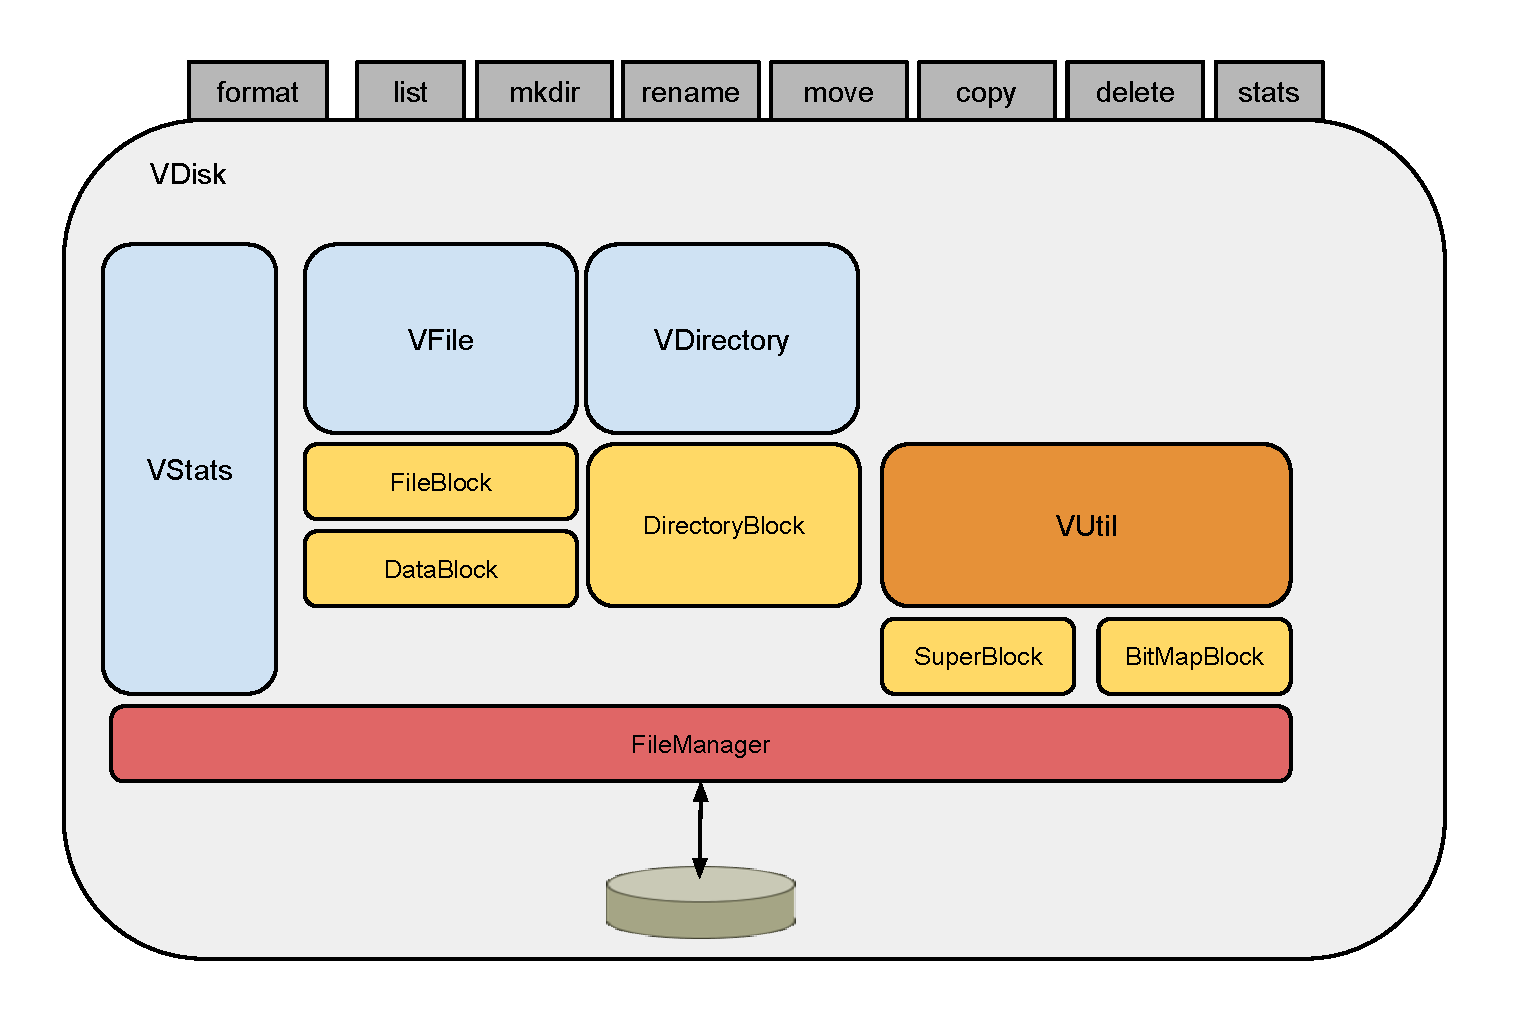
\includegraphics[scale=0.4]{images/AVDisk.pdf}
\caption{Illustration of VDisk}
\label{abstactVdisk}
\end{center}
\end{figure}

\subsubsection{VFS File Format}
A formatted \emph{VFS file} has a fixed-size header, which consists of a super block (represented by the previously mentioned \texttt{SuperBlock} class, a bitmap block (\texttt{BitMapBlock} and a single directory block (\texttt{DirectoryBlock}) called \texttt{rootDirectoryBlock}. The layout is visible in figure (\ref{vdiskheader}).

\begin{figure}[h]
\begin{center}
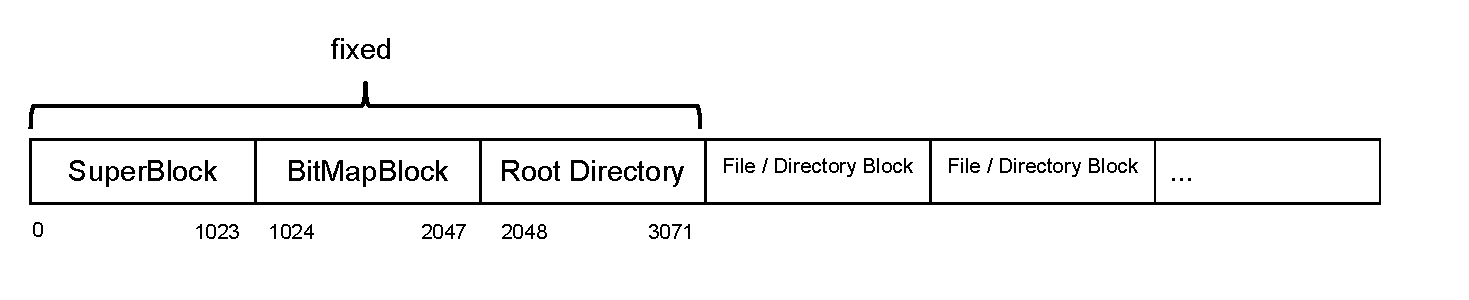
\includegraphics[scale=0.6]{images/VDiskHeader.pdf}
\caption{first three Blocks of a VDisk file}
\label{vdiskheader}
\end{center}
\end{figure}

\begin{figure}[h]
\begin{center}
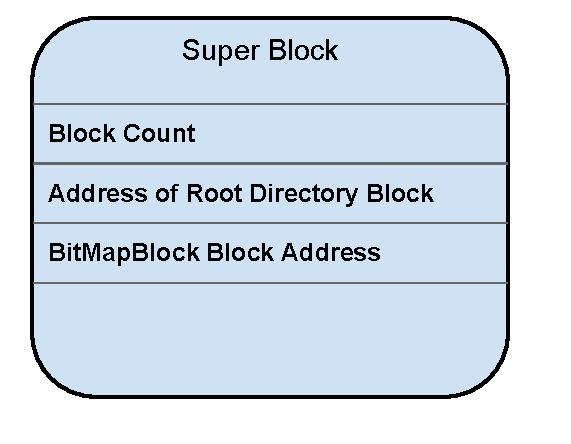
\includegraphics[scale=0.5]{images/SuperBlock.pdf}
\caption{representation of our SuperBlock, which contains all necessary properties of the VFS}
\label{superblock}
\end{center}
\end{figure}

\begin{figure}[h]
\begin{center}
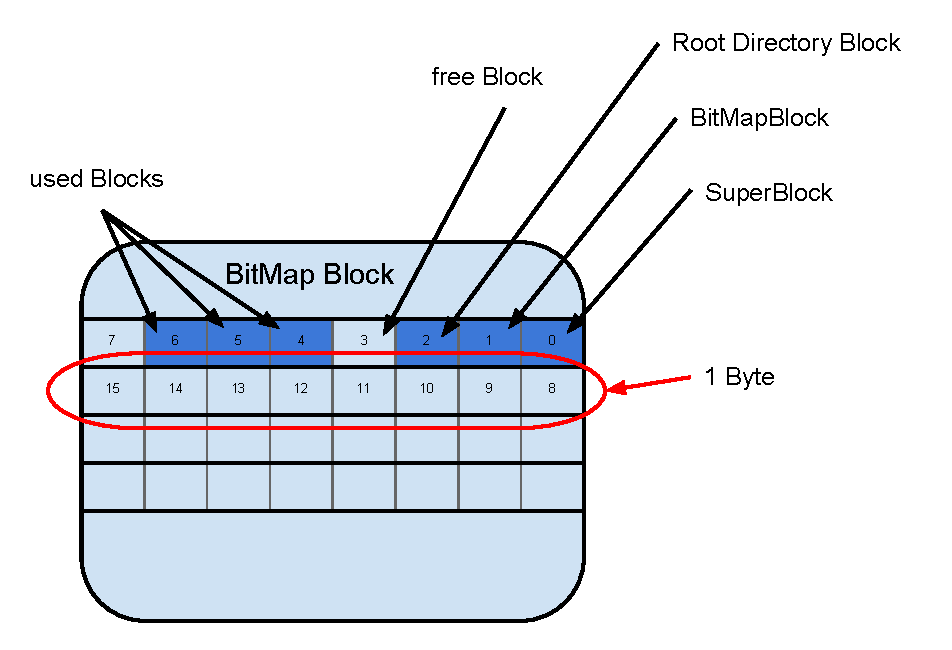
\includegraphics[scale=0.5]{images/BitMapBlock.pdf}
\caption{representation of our BitMapBlock which keeps track of the used and free block of the VFS}
\label{bitmapblock}

\end{center}
\end{figure}


\begin{figure}[h]
\begin{center}
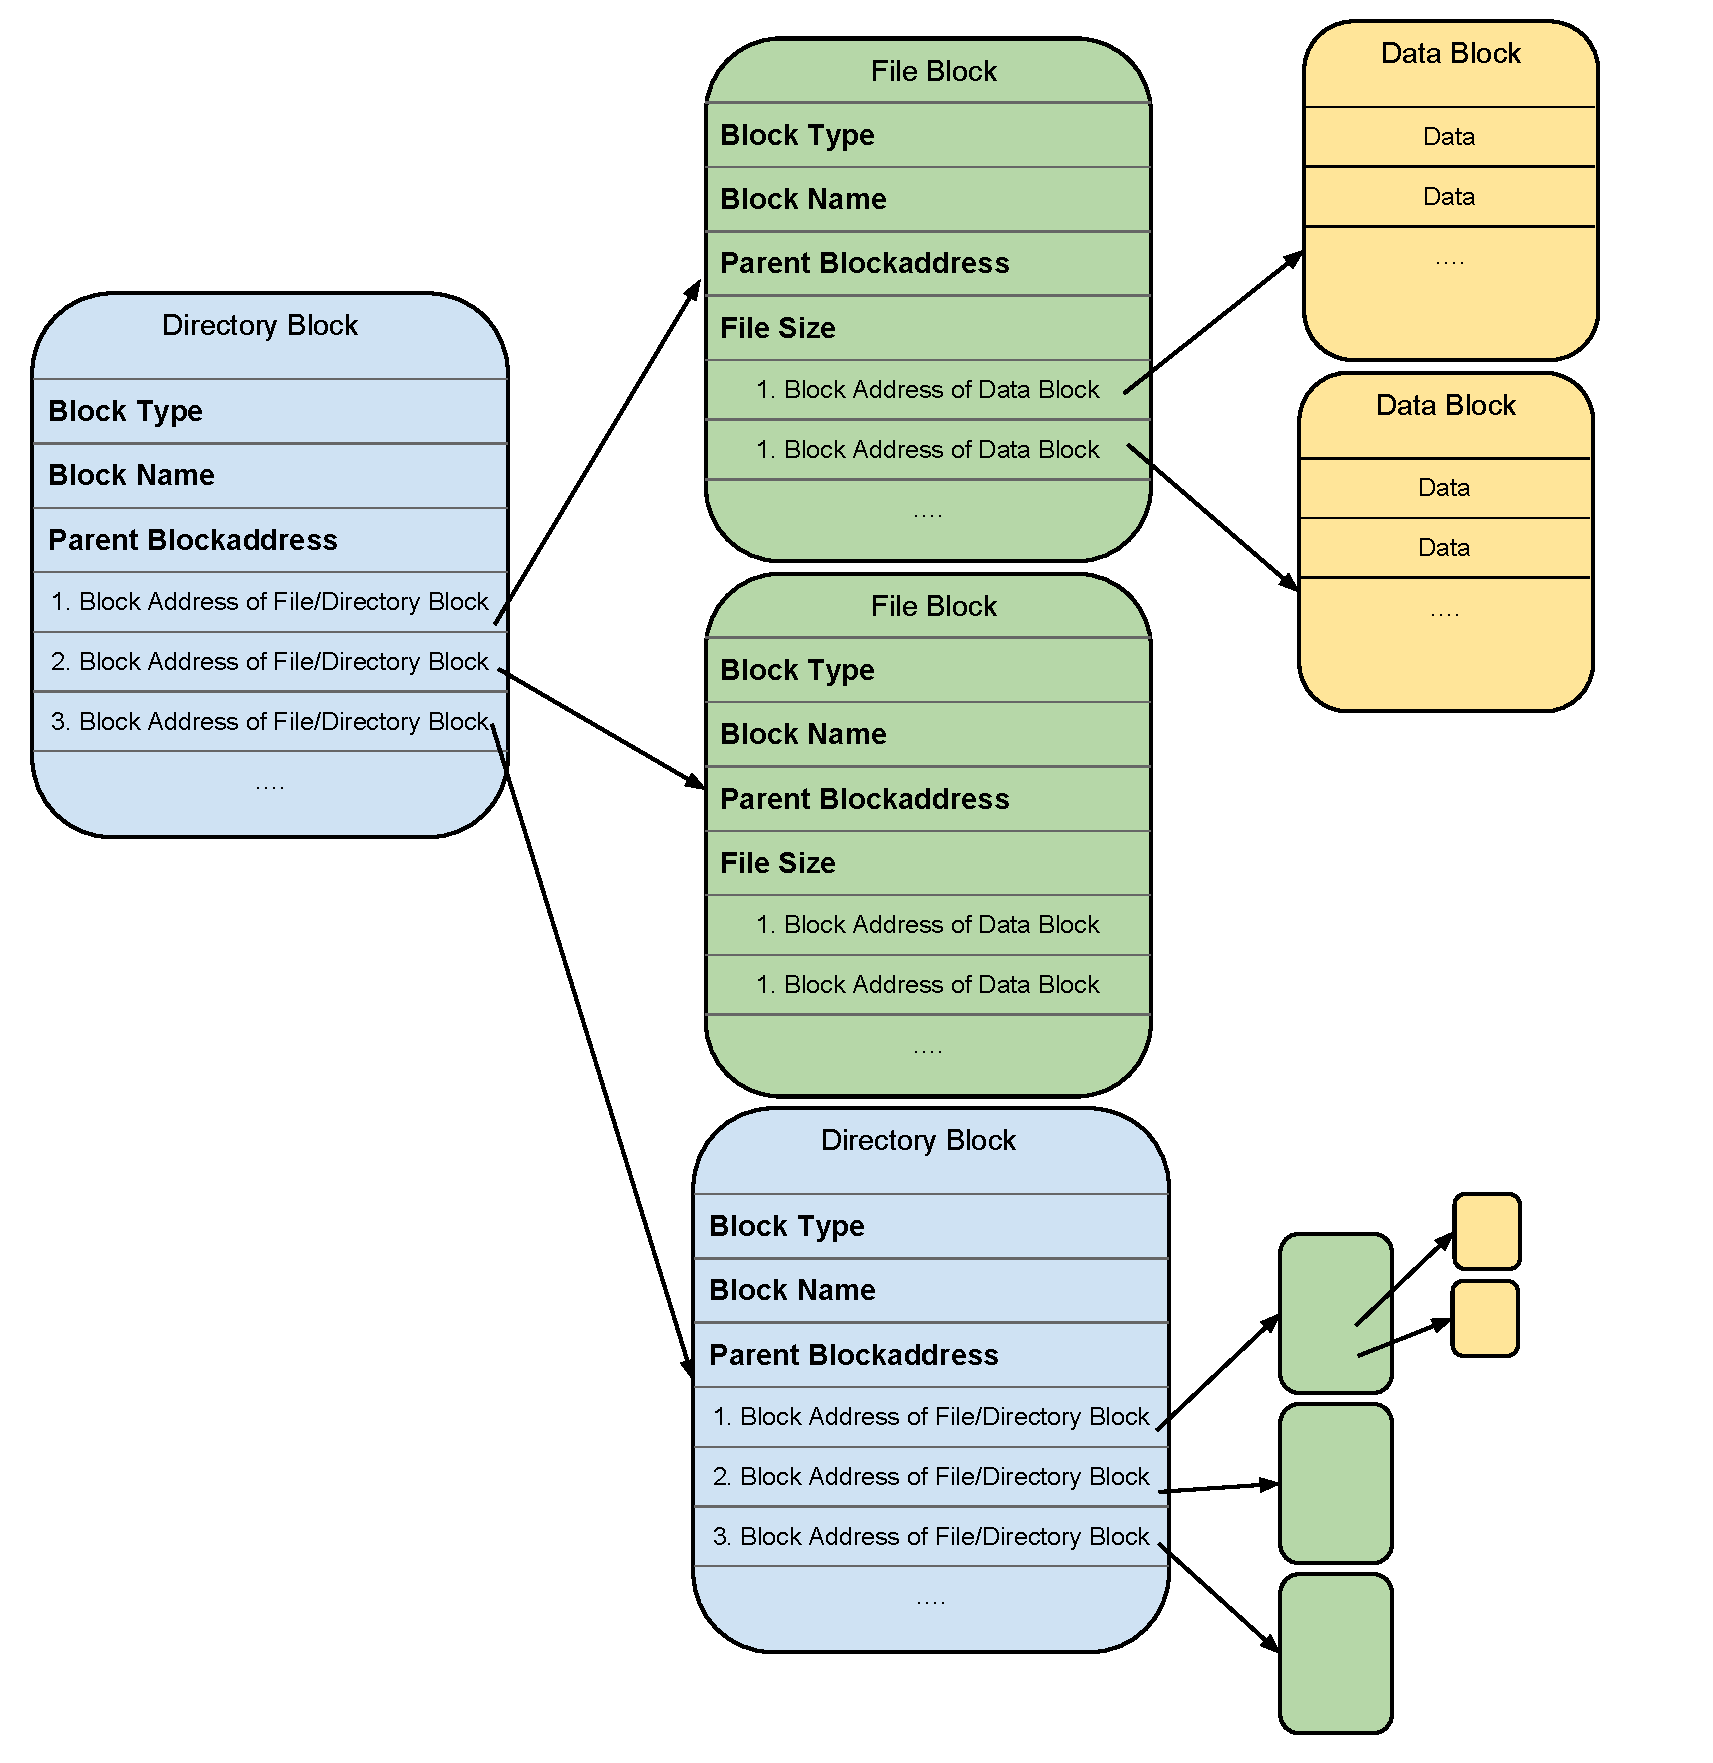
\includegraphics[scale=0.3]{images/Blocks.pdf}
\label{blocks}
\caption{Schematically illustration how the blocks are arranged}
\end{center}
\end{figure}


\subsubsection{Design Patterns}

% START multiline comment
\ifx true false


% PART II: VFS Browser
% --------------------------------------

\section{VFS Browser}

% TODO: Remove this line
\textbf{[This section has to be completed by April 22nd.]}

%TODO: Remove this text and replace it with actual content
\emph{Give a short (1-2 paragraphs) description of what VFS Browser is.}


\subsection{Requirements}

% TODO: Remove this text and replace it with actual content
\emph{Describe which requirements (and possibly bonus requirements) you have implemented in this part. Give a quick description (1-2 sentences) of each requirement. List the software elements (classes and or functions) that are mainly involved in implementing each requirement.}


\subsection{Design}

% TODO: Remove this text and replace it with actual content
\emph{Give an overview of the design of this part and describe in general terms how the implementation works. You can mention design patterns used, class diagrams, definition of custom file formats, network protocols, or anything else that helps understand the implementation.}


\subsection{Integration}

% TODO: Remove this text and replace it with actual content
\emph{If you had to change the design or API of the previous part, describe the changes and the reasons for each change here.}



% PART III: Synchronization Server
% --------------------------------------

\section{Synchronization Server}

% TODO: Remove this line
\textbf{[This section has to be completed by May 13th.]}

%TODO: Remove this text and replace it with actual content
\emph{Give a short (1-2 paragraphs) description of what VFS Browser is.}


\subsection{Requirements}

% TODO: Remove this text and replace it with actual content
\emph{Describe which requirements (and possibly bonus requirements) you have implemented in this part. Give a quick description (1-2 sentences) of each requirement. List the software elements (classes and or functions) that are mainly involved in implementing each requirement.}


\subsection{Design}

% TODO: Remove this text and replace it with actual content
\emph{Give an overview of the design of this part and describe in general terms how the implementation works. You can mention design patterns used, class diagrams, definition of custom file formats, network protocols, or anything else that helps understand the implementation.}


\subsection{Integration}

% TODO: Remove this text and replace it with actual content
\emph{If you had to change the design or API of the previous part, describe the changes and the reasons for each change here.}

% END multiline comment
\fi

% PART IV: Quick Start Guide
% --------------------------------------

\section{Quick Start Guide}

% TODO: Remove this line
\textbf{[optional: This part has to be completed by April 8th.]}

% TODO: Remove this text and replace it with actual content
\emph{If you have a command line interface for your VFS, describe here the commands available (e.g. ls, copy, import).} \\ \\ \\

% START multiline comment
\ifx true false

% TODO: Remove this line
\noindent\textbf{[This part has to be completed by May 13th.]}

% TODO: Remove this text and replace it with actual content
\emph{Describe how to realize the following use case with your system. Describe the steps involved and how to perform each action (e.g. command line executions and arguments, menu entries, keyboard shortcuts, screenshots). The use case is the following:
\begin{enumerate}
\item Start synchronization server on localhost.
\item Create account on synchronization server.
\item Create two VFS disks (on the same machine) and link them to the new account.
\item Import a directory (recursively) from the host file system into Disk 1.
\item Dispose Disk 1 after the synchronization finished.
\item Export the directory (recursively) from Disk 2 into the host file system.
\item Stop synchronization server.
\end{enumerate}
}

% END multiline comment
\fi

\end{document}
